\subsubsection{الگوی \lr{Monitor-Actuator}}
\label{archSafeMonActSec}
\begin{RTL}
این الگو \cite{ref4} یک راهکار ایمنی مقرون‌به‌صرفه است که در سیستم‌هایی
با نیازمندی‌های دسترسی متوسط تا پایین و حالت ایمن تعریف‌شده استفاده می‌شود.
این الگو شامل یک حسگر مستقل است که کانال فعال‌سازی
را برای شناسایی خطاها نظارت می‌کند و اطمینان می‌دهد که
سیستم در صورت لزوم به حالت ایمن وارد می‌شود. این الگو شکل
خاصی از \nameref{archSafeHeteroRedundancySec} است که به جای تکرار
کامل کانال، نظارت را فراهم می‌کند. زمانی که سیستم می‌تواند با ورود
به حالت ایمن، خطاها را تحمل کند، مناسب است و
با کمترین تکرار اطمینان حاصل می‌شود که اگر یک کانال خراب شود،
کانال دیگر می‌تواند خطا را شناسایی کرده یا به کار خود ادامه دهد.
\end{RTL}
\begin{figure}[h!]
\centering
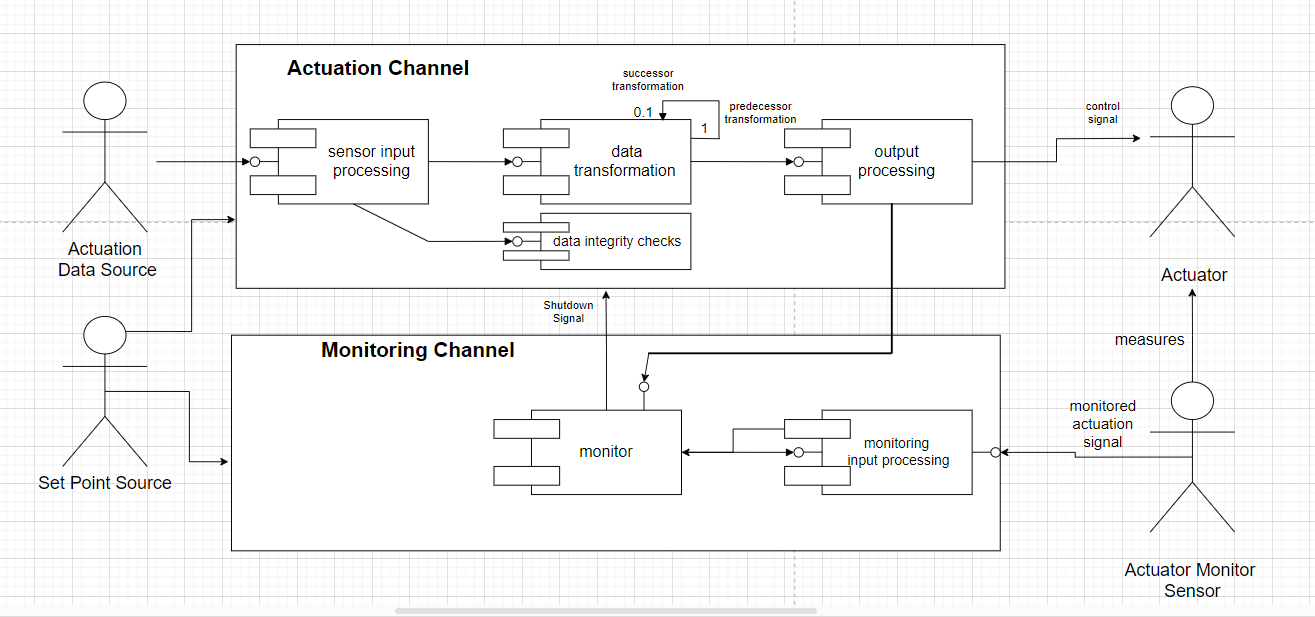
\includegraphics[scale=0.5]{images/third/monitorActuator.png}
\caption{ساختار الگوی \lr{Monitor Actuator}}
\end{figure}